% 同时的相对性
\begin{figure}[htbp]
    \centering
    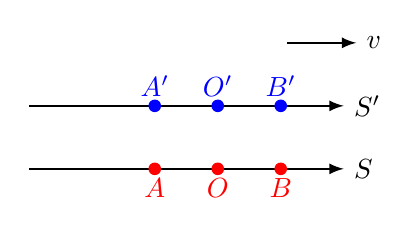
\begin{tikzpicture}[scale=0.8, >=latex]
        \draw [thick, ->] (1,0) -- (6,0) node [right] {$S$};
        \draw [thick, ->] (1,1) -- (6,1) node [right] {$S'$};
        
        \draw [thick, ->] (5.1,2) -- (6.2,2) node [right] {$v$};
        
        \fill [red] (3,0) circle (0.1) node [below] {$A$};
        \fill [red] (4,0) circle (0.1) node [below] {$O$};
        \fill [red] (5,0) circle (0.1) node [below] {$B$};
        
        \fill [blue] (3,1) circle (0.1) node [above] {$A'$};
        \fill [blue] (4,1) circle (0.1) node [above] {$O'$};
        \fill [blue] (5,1) circle (0.1) node [above] {$B'$};
    \end{tikzpicture}
    \caption{「同时」的相对性}
    \label{fig:simultaneity}
\end{figure}